\documentclass[conference]{IEEEtran}
\usepackage{cite}
\usepackage{graphicx}
\usepackage{multirow}
\usepackage{amssymb}
\usepackage{siunitx}
\usepackage{dcolumn}
\usepackage{color, colortbl}
\usepackage{balance}
\usepackage{caption}
\usepackage{url}
\usepackage{subcaption}
\definecolor{Gray}{gray}{0.9}


\clubpenalty = 10000
\widowpenalty = 10000
\displaywidowpenalty = 10000

% correct bad hyphenation here
\hyphenation{op-tical net-works semi-conduc-tor}



\begin{document}
%
% paper title
% Titles are generally capitalized except for words such as a, an, and, as,
% at, but, by, for, in, nor, of, on, or, the, to and up, which are usually
% not capitalized unless they are the first or last word of the title.
% Linebreaks \\ can be used within to get better formatting as desired.
% Do not put math or special symbols in the title.
\title{Flower: Navigating Program Flow in the IDE}


% author names and affiliations
% use a multiple column layout for up to three different
% affiliations
\author{\IEEEauthorblockN{Chris Brown, Justin Smith, Tyler Albert, and Emerson Murphy-Hill}
\IEEEauthorblockA{Department of Computer Science\\
North Carolina State University\\
Raleigh, North Carolina 27606\\
Email: \{dcbrow10, jssmit11, tralber2\}@ncsu.edu, emerson@csc.ncsu.edu}
}

% make the title area
\maketitle

% As a general rule, do not put math, special symbols or citations
% in the abstract
\begin{abstract}
Program navigation is a critical task for software developers. 
%Many tools and approaches have been proposed to aide developers in navigating programs.
%In this work we present a tool, Flower, that enables developers 
The current state-of-the-art tools support program navigation by leaning heavily on visualizations and cumbersome interface widgets.
To assist developers in effectively navigating program flow, we designed and implemented a new tool that leverages program analysis techniques while maintaining a minimalistic interface.
Our tool enables developers to simultaneously navigate control flow and data flow within the Eclipse Integrated Development Environment (IDE).
Based on a preliminary evaluation with 8 programmers, our tool succeeds when call graphs contained relatively few branches, but was strained by complex program structures. 
%We present a different way to do things... enable the navigation control flow and data flow simultaneously using minimal interface alterations.
%Something about tradeoffs.
%For simple sub-tasks tool was effective with very few interface elements. 
\end{abstract}

% no keywords



\IEEEpeerreviewmaketitle


\section{Introduction}
Modern software systems contain millions of lines of source code. 
As software grows in size and complexity, developers increasingly rely on tools to help them navigate the programs they create. 
A software testing study described a wide variety of tools developers use to validate their code, but also found that inadequate testing and debugging tools contributed to poor quality software in production\cite{NIST-02-3}.

Finding, comprehending, and fixing bugs has become the most common software activity, consuming 70-80\% of software engineers' time~\cite{Whyline}. 
Program navigation can help improve developers' program comprehension, which Brooks argues is vital because this type of domain-specific knowledge plays a key role in nearly every software task including development, code reviews, debugging, code maintenance, and testing~\cite{BrooksComprehension}. 

Although integrated development environments (IDEs) present code linearly in the order methods are defined in a file, successful developers do not navigate source code line by line starting at the top of the file. 
Instead, they methodically navigate the code's hierarchical semantic structures~\cite{robillard2004investigate}.
While navigating programs, developers ask questions about control flow and data flow throughout the program~\cite{latoza2010hard, Smith2015}. 
We will refer to these two concepts together as \textit{program flow}. 

To realize their ideal program flow navigation strategies, developers rely on navigation tools that expose the links between sometimes distant locations in the source code. 
Many existing tools do so by displaying call graph visualizations or adding views to the the screen.
In general, evaluations have demonstrated the effectiveness of such tools ~\cite{Reacher,Whyline,Relo,Stacksplorer}.

However, these tools rely on cumbersome user interface widgets that new users might struggle to understand and occupy valuable screen real estate.
We present a tool, Flower (pronounced flow-er), that represents a minimalistic approach to program navigation.
Flower  leverages program analysis techniques, leans on relatively few cumbersome interface elements, and presents its results integrated within the code.
%Existing tools feature many cumbersome UI widgets or seem poorly integrated into the IDE.
%Previous approaches help developers navigate control flow by helping them visualize. 
%The additional graphs, maps, and visualizations have been shown to help developers stay oriented. However, (occupy a lot of screen real estate, may be difficult for new users to understand, mapping stuff). 
%Also, don't help developers navigate both flows at the same time.   

%This paper makes the following contributions:

Consider the following motivating example involving Hillary, a professional Java developer at a large software company.
While maintaining some old code, Hillary notices a warning from a static analysis tool --- this variable contains user-provided data. 
If it is used in a sensitive context before being sanitized, this code could be vulnerable to security vulnerabilities.

Hillary sets out to determine if the variable is sanitized on all paths leading to the sensitive context.
She vaguely recalls using an Eclipse tool to help her trace control flow through a program, but is unsure how to invoke it or whether it also traces data flow.
She looks through various menus, tries out a few tools, but cannot locate the right tool.
Turning her attention back to the code, she begins scrolling through the current file, unknowingly using Eclipse's \emph{Mark Occurrences} tool while scanning for uses of the variable. 
After inspecting all the occurrences in the current file, she now begins searching for methods that take the variable as input.
She stumbles upon Eclipse's \emph{Call Hierarchy} tool, which seems helpful, but she is unable to specify the variable she is interested in when invoking the tool.

Undeterred, she finds a method that takes the variable as a parameter and invokes \emph{Call Hierarchy} on that method.
Eclipse opens a new view containing \emph{Call Hierarchy's} representation of the call graph.
Hillary continuously switches back and forth between the \emph{Call Hierarchy} view and the code.
She uses the \emph{Call Hierarchy} view to navigate chains of method calls and inspects the code in each method to check whether the variable gets sanitized correctly.
She repeats this process for a few more call sites, but grows fatigued. 
Unsure of whether the the variable gets sanitized along all paths, she decides to ignore the warning.
Two months later an attacker exploits the vulnerability, costing her company hundreds of millions of dollars. 
Hillary gets fired for her oversight. 
%Without her high-paying job, she can no longer afford to feed her kids and pay her mortgage. Drowning in credit card debt, homeless, and divorced, Hillary curses the Eclipse tools that let her down.   
Though Hillary is fictional, her story is based on the experiences of real developers we observed in a previous study~\cite{Smith2015}.

The contribution of this work is the design, implementation, and evaluation of a new program navigation tool, Flower.
As we will discuss, Flower  addresses many of the types of issues that Hillary faced by implementing four key design principles (Section \ref{DesignPrinciples}).
We evaluate Flower, to better understand what types of tasks it effectively supports. 
In contrast to existing navigation tools, Flower  enables developers to simultaneously trace data flow and control flow within the code view. 


\section{Design Principles}
\label{DesignPrinciples}
In this section we describe the design principles that we used to shape Flower. We derived these design principles from a previous study \cite{Smith2015} and by examining existing program navigation tools.
 
\vspace{1em} 
\noindent\textbf{Program Analysis} ---
Simple textual analysis may lead to inaccurate results in many scenarios. For example, such analysis fails when programs include duplicated variable names that refer to different variables in different scopes. Textual analysis also falls short when programs contain inheritance and when variable names are included in comments, documentation, or other syntactically irrelevant locations.
By leveraging program analysis techniques, navigation tools can provide more accurate information than simple textual analysis.
By analyzing abstract syntax trees (ASTs) and call graphs, tools can make references to relevant variables and methods. 

\vspace{1em} 
\noindent\textbf{Low Barriers to Invocation} ---
Some tools are easier to invoke than others. 
Take Hillary's case for example.
She easily invoked \emph{Mark Occurrences}, but initially struggled to locate and invoke \emph{Call Hierarchy}.
Tools with high barriers to invocation require users to sift through menus and include unintuitive widgets. 
Barriers to invocation inhibit adoption~\cite{johnson2013don}.
As developers navigate multiple program paths concurrently, repetitively invoking tools may be cumbersome, especially if barriers are high. 


\vspace{1em} 
\noindent\textbf{Full Program Navigation}  ---
Developers are not only interested in traversing programs' call graphs, but also how data flows through the call graph~\cite{Smith2015}.
To do so, developers must inspect the relationship between methods as well as the methods themselves.
Often the methods of interest span across multiple source files.
For Hillary, \emph{Mark Occurrences} helped her navigate a single file, but fell short when she wanted to inspect methods in other files.
Furthermore, program navigation tools should support this traversal both upstream and downstream. 
That is, tools should highlight variable assignments and also subsequent variable uses. 

\vspace{1em} 
\noindent\textbf{In Situ Navigation}  ---
Switching between views in the IDE can cause disorientation~\cite{deAlwis2006disorient}. 
As developers navigate through code, navigation tools should present their results in that context. 
This was a problem for Hillary, who had to constantly switch between the \emph{Call Hierarchy} view and the code view.
When navigation tools present results outside the code, developers are burdened with the cognitive load of translating those results back to the code.

\section{Related Work}
%Summary of related work, including a table evaluating existing %tools on various design principles.
%Spoiler alert, none of the tools satisfy all of the principles.
Here we discuss many of the various existing tools that help developers explore and navigate code. We also relate the exiting tools back to Design Principles Described in Section \ref{DesignPrinciples}.

Many modern IDEs provide tools that help developers navigate through their code. 
For example, Eclipse~\cite{Eclipse} includes \emph{Call Hierarchy} and \emph{Find References}. 
When users invoke \emph{Call Hierarchy}, Eclipse opens a new view that displays the callers and callees for a selected method.  
IntelliJ~\cite{IntelliJ} also provides navigation tools, namely \emph{Analyze Data Flow To/From Here} and \emph{Analyze Dependencies}.
Much like Eclipse's \emph{Call Hierarchy}, the \emph{Analyze Data Flow} tools display their results in external views. 
These tools provide \textit{Program Analysis} for users to navigate throughout the entirety of a project. 
However, they generally differ from Flower because they lack \textit{Low Barriers to Invocation} and \textit{In Situ Navigation}.

There are also several tools that reside strictly within the code editor, enabling a form of \textit{In Situ Navigation}.
Two examples of these tools are Eclipse's \emph{Mark Occurrences} and \emph{Open Declaration}. 
Eclipse automatically invokes \emph{Mark Occurrences} whenever a user clicks on a variable or method name in the code.
The tool then highlights occurrences of that element elsewhere in the current file.
\emph{Mark Occurrences} epitomizes \textit{Low Barriers to Invocation}.
These approaches are similar to Flower  in that they display the results within the editor rather than a separate view or panel.
However, they do not provide \textit{Program Analysis} or enable \textit{Full Program Navigation}.


Many other tools help developers navigate code by representing the code graphically and allowing developers to navigate those graphs~\cite{CodeBubbles,CodeCanvas,CodeSurfer,Dora,Reacher,Relo,Whyline}. 
These works provide various views of control flow graphs, class and UML-like diagrams, trees, call graphs, and other images to describe the hierarchy and relationship between different variables or functions within the code. 
To generate accurate visualizations, these types of tools utilize \textit{Program Analysis}.
Additionally, most of these tools implement some aspects of \textit{Full Program Navigation}.
Flower differs because from these tools in the way it presents results (\textit{In Situ Navigation}) and because it has \textit{Low Barriers to Invocation}.

%\begin{table}
%	\centering
%	\caption{Design Principles}
%	\begin{tabular}{r|c|c|c|c}
%		\rowcolor{Gray}
%		\hline
%		Tools & & Low & Full Prog. & In Situ\\
%		\rowcolor{Gray}
%		 & Analysis & Barriers & Nav. & Nav.\\
%		\hline
%		Call Hierarchy & \checkmark & - & \checkmark & -\\
%		\rowcolor{Gray}
%		Find References & \checkmark & - & \checkmark & -\\
%		Analyze Data Flow & \checkmark & - & \checkmark & -\\
%		\rowcolor{Gray}
%		Analyze Dependencies & \checkmark & - & \checkmark & -\\
%		Mark Occurrences & - & \checkmark & - & \checkmark \\
%		\rowcolor{Gray}
%		Open Declaration & \checkmark & - & \checkmark & \checkmark \\
%		Code Bubbles & \checkmark & - & \checkmark & \checkmark \\
%		\rowcolor{Gray}
%		Code Canvas & \checkmark & - & \checkmark & \checkmark \\
%		Code Surfer & \checkmark & - & \checkmark & Sometimes \\
%		\rowcolor{Gray}
%		Dora & \checkmark & - & \checkmark & - \\
%		Reacher & \checkmark & - & \checkmark & - \\
%		\rowcolor{Gray}
%		Relo & \checkmark & - & \checkmark & - \\
%		Whyline & \checkmark & - & \checkmark & - \\
%		\hline
%	\end{tabular}
%	\label{table:background}
%\end{table}
%

\begin{figure*}
	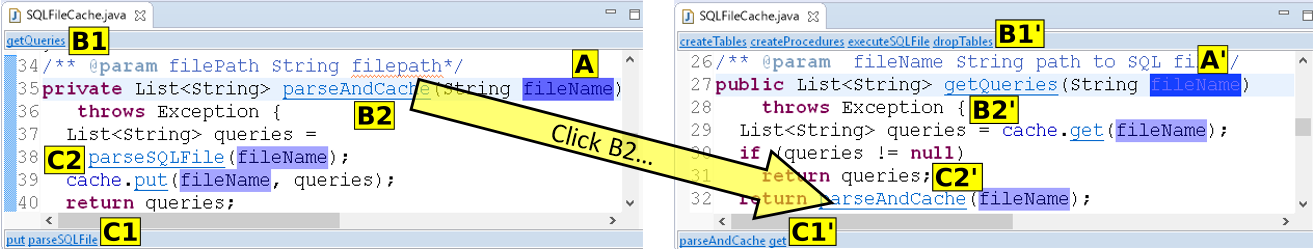
\includegraphics[width=\textwidth]{images/toolScreenshot}
	\caption{Code view in the Eclipse IDE with Flower invoked during Task 1. The image on the left shows the tool running in the method \texttt{parseAndCache}. When the user clicks on the link in the editor (B1 or B2), they are taken to the function \texttt{getQueries}, which is a caller of \texttt{parseAndCache}.}	
	\label{fig:tool} 
\end{figure*}

\section{Flower}
Flower was designed to realize all of the principles described in Section \ref{DesignPrinciples}. 
We implemented Flower as a plugin to the Eclipse IDE~\cite{Eclipse}. 
We chose Eclipse because it is one of the most widely used open source IDEs for Java development and it provides many extension points for plugins. 

Figure \ref{fig:tool} depicts Flower invoked on a variable participants were asked to inspect as part of our evaluation. To visualize how a programmer would interact with Flower, consider the following scenario:


Suppose you are a programmer and you notice that by tampering with the value of the \texttt{fileName} variable, malicious users could gain access to sensitive information in the database. 
You want to determine whether users can modify \texttt{fileName} before it gets passed into \texttt{parseAndCache}. 
First, you click on \texttt{fileName} (A).
Much like \emph{Mark Occurrences}, Flower is automatically invoked.
To help you locate where the variable is modified and referenced, Flower highlights occurrences of that variable in the code.
Since \texttt{fileName} is a formal parameter to \texttt{parseAndCache}, any method calling \texttt{parseAndCache} could modify \texttt{fileName}. 
Those methods reside in other files, so Flower  provides links to their locations (B1).
Rather than move your mouse up to the top of the editor window, you click on \texttt{parseAndCache} (B2), which conveniently links to the first call site, \texttt{getQueries}. 
Flower  opens \texttt{getQueries} and highlights the location in that method where \texttt{fileName} passed to \texttt{parseAndCache} and shows that the value is passed to \texttt{getQueries} from \texttt{createTables}, \texttt{createProcedures}, \texttt{executeSQLFile}, and \texttt{dropTables} as seen in Fig. \ref{fig:tool}.  

%Something about using Flower for down flow.
%(A) - When a user clicks on a variable all (visible) instances of that variable are highlighted in the code. (B) - When the variable has been declared as a parameter to the current method, users can click on that method's name in the editor to navigate to a location where that method is called. (X) - When the variable is passed to an external method, users can click on that method's name to open its declaration. (C) - If the variable is passed in from another method or is defined earlier in the current file, a link to that location is displayed in the ``top box.'' (D) - If the variable is passed in to another method or referenced later in the current file, links to those locations appear in the ``bottom box.''


\section{Preliminary Evaluation}
We performed a preliminary evaluation of Flower with eight programmers performing two code navigation tasks.\footnote{Materials available online at \url{tinyurl.com/flowerTool}}
As a baseline, we compare our tool against the existing suite of tools available in Eclipse (\emph{Open Declaration}, \emph{Mark Occurrences}, and \emph{Call Hierarchy}).
Our goals in this study were to (a) determine what types of navigation activities Flower  effectively supports and fails to support and (b) get feedback on the usability of Flower.
To answer (a), we measured how quickly and accurately participants completed different activities.
The remainder of this section describes our participants, study design, and task selection, and concludes with our approach to answer (b).

All participants were graduate students at the time of the study with a mean of 5 years of professional programming experience; Table \ref{table:participants} provides additional information about each participant. We recruited participants using a convenience sampling approach. 
Before the study, we asked participants to report whether they were familiar with the Eclipse IDE. This information helped us balance Eclipse novices across groups.

Each participant used Flower for one task and Eclipse's tools for the other task.
To control for learning and fatigue effects, we permuted the order participants received each tool and performed each task. 
Each participant was assigned to one of four groups (Task Group column in Table \ref{table:participants}).



We based our tasks in this study on two tasks (Tasks 1 and 3) from a previous study ~\cite{Smith2015}.
In the previous study, participants used a think-aloud protocol to, among other things, describe their program navigation strategies.
Here, we did not interrupt, prompt, or ask participants to think aloud until after they had completed the tasks as to not distort their task completion time.

The two tasks we chose are complementary in that Task 1 required participants to navigate up the call graph, inspecting the callers of the initial method. 
On the other hand, Task 2 required participants to inspect the methods called by the initial method.
For Task 1 we asked participants to tell us whether a method ever receives user-provided input.
For Task 2 we asked participants to tell us whether a form field is validated before being sent to the database.
To ensure all participants had a baseline familiarity, we trained participants on the appropriate tools preceding each task. 
To evaluate the effectiveness of the navigation tools rather than participants' familiarity with a particular code base, we asked participants to navigate code they had not previously contributed to. 

%We chose two tasks that (differentiate between the two tasks... up and down?)

To evaluate the usability of Flower, we administered an adapted version of the Post-Study System Usability Questionnaire (PSSUQ)~\cite{Lewis95ibmcomputer} after participants had completed both tasks. We modified the questionnaire by replacing ``this system'' with ``this tool'' and asked questions from the System Quality and Interface Quality categories.
To prompt discussion about the usability of Flower, we also asked participants open-ended questions based on applicable categories from Nielsen's usability heuristics~\cite{Nielsen1992}.
%To capture participant's experiences that these two metrics overlooked, two of the authors independently examined each audio/video recording and recorded memos. 


\section{Results}
Here we present the results of our preliminary evaluation. 
We present our results thematically to illustrate the types of activities Flower  effectively supported.

%\begin{figure}
%	\centering
%	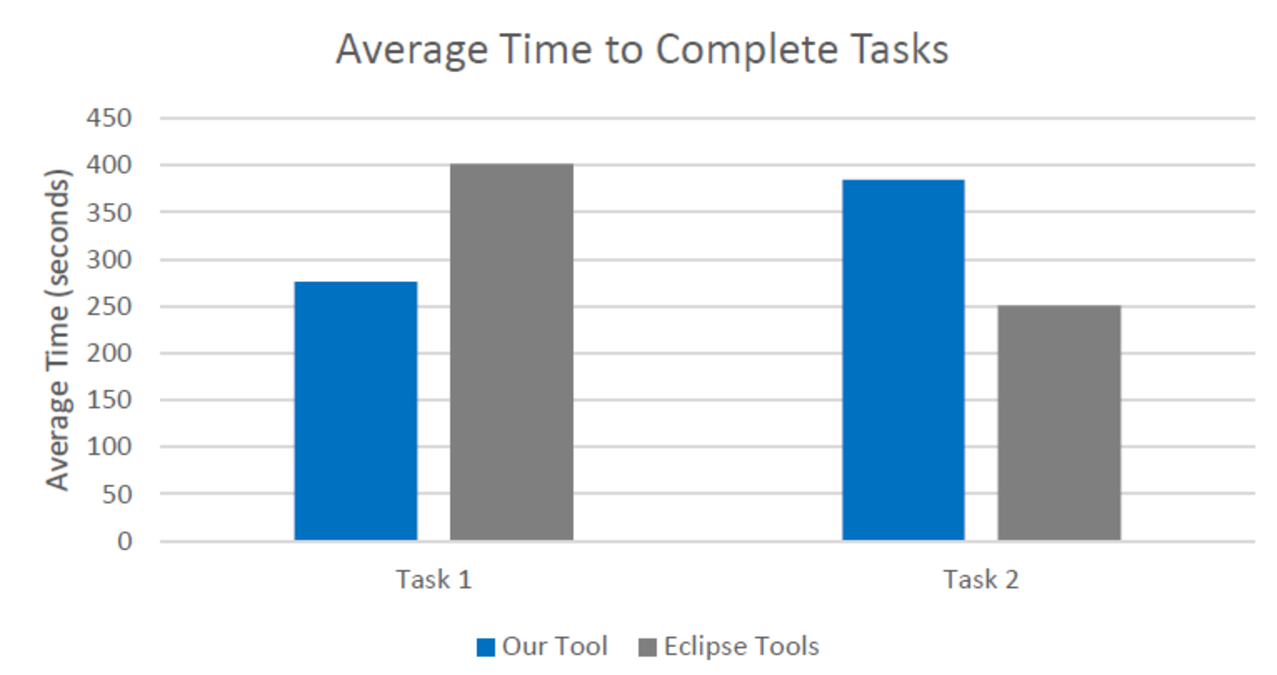
\includegraphics[width=\columnwidth]{images/taskTime}
%	\caption{Mean time to complete each task with and without Flower}
%	\label{fig:taskTime} 
%\end{figure}

\textbf{Approachable Interface:}
Compared to other PSSUQ questions, participants responded most positively to the three questions about Flower's simplicity, how easy it was to use, and how easy it was to learn. 
These responses seem to indicate that participants were most enthusiastic about Flower's minimalistic interface. 
Participants reiterated these sentiments in their responses to the open-ended questions. 
For the most part, participants felt it was easy to remember how to use Flower and that it featured a ``consistent interface.''

\textbf{Branchless Navigation:}
For Task 1, all participants correctly navigated up the call graph and did so faster with Flower  compared to the Eclipse tools.
With Flower, participants' mean completion time was 276 seconds, compared to 402 seconds with the Eclipse tools.

The first two steps in this task involved navigating a portion of the call graph that did not include any branches.
In other words, participants started in the \texttt{parseSQLFile} method, which was only called in one location, \texttt{parseAndCache}. 
The \texttt{parseAndCache} method was only called in one method \texttt{getQueries}.
Participants equipped with our tool were strictly faster in navigating the first step up this branchless chain. 
The mean times for participants to reach \texttt{parseAndCache} with Flower and the Eclipse tools were 8 seconds and 44 seconds, respectively.
These two results suggest that Flower successfully adhered to the \textit{Low Barriers to Invocation} design principle. 

\textbf{Branching and Backtracking:}
For Task 2, participants were more accurate with Flower.
Two participants (P3 and P6) navigated to the correct validation method with Flower.
Only one (P8) did so with the Eclipse tools.

However, the mean completion time for Task 2 with Flower was higher (385 seconds) compared to the Eclipse tools (251 seconds).
Additionally, participants who used Flower  for Task 2 scored the tool lower on the PSSUQ than those who used it for Task 1.
Based on open-ended responses and our observations of participants, we provide one likely explanation for this deficiency.
Participants were required to sift through more variable references and method calls to complete Task 2.
In navigating this more complex program structure, when participants took missteps they found it difficult to backtrack.
While working on Task 2 with Flower P6 attempted to use Eclipse's built-in back buttons to backtrack, but still had difficulty reorienting himself. 
To a lesser extent, we observed this same difficulty during Task 1.
After navigating through several chains of method invocations with Flower, P7 felt like she had reached a ``dead end'' and was unsure of how to navigate back to where she came from.
Similarly, after reaching a top-level method, P1 asked, ``How can I return back to where I came from?''

%PSSUQ responses support this. Could talk about the low categories
%On the other hand, participants responded most negatively to questions about whether the tool provided all the expected functions and capabilities and whether it would enable them to complete tasks quickly.
%All the functions I expected (Missing tracability and mark bars, ... )
%To these two questions, participants' median response was 5. 


%Overall, task competion time distorts the actual time participants took to complete the task.
%Participants who explored more of the call graph are penalized. 
%Some participants spent additional time exeploring after finding the right answer to confirm their conclusion

%(Not sure how to report correctness here... 4 gave the correct answer with eclipse tools --
%2 were correct with ours. However, the incorrect two navigated correctly, located a hard-coded %parameter, responded incorrectly, and did not justify)
%However, participants were Y\% slower for Task 2.
%(Correctness in terms of navigation was even split. One with our tool guessed correctly)

%To understand why participants were faster for Task 1 with Flower, we analyzed how long it took participants to navigate one step up the call graph. 

%DFS exploration stategies


\begin{table}
	\centering
	\caption{Participant Demographics}
	\begin{tabular}{cSScc}
		\rowcolor{Gray}
		\hline
		\multicolumn{1}{c}{\textbf{Participants}} & \multicolumn{1}{c}{\textbf{Industry}} & \multicolumn{1}{c}{\textbf{Java}} &\multicolumn{1}{c}{\textbf{Eclipse}} & \multicolumn{1}{c}{\textbf{Task}} \\
		\rowcolor{Gray}
		\multicolumn{1}{c}{ } & \multicolumn{1}{c}{\textbf{Exp.} \textit{(years)}} & \multicolumn{1}{c}{\textbf{Exp.} \textit{(years)}} & \multicolumn{1}{c}{\textbf{Exp.}} & \multicolumn{1}{c}{\textbf{Group}}\\
		\hline
		P1 & 9 & 5 & \checkmark & T1* - T2 \\
		\rowcolor{Gray}
		P2 & 0 & 6 & \checkmark & T2* - T1\\
		P3 & 3 & 2 & - & T1 - T2*\\
		\rowcolor{Gray}
		P4 & 5 & 0 & - & T2 - T1*\\
		P5 & 12 & 10 & \checkmark & T1* - T2\\
		\rowcolor{Gray}
		P6 & 0 & 3.5 & \checkmark & T2* - T1\\
		P7 & 1 & 9 & \checkmark & T1 - T2*\\
		\rowcolor{Gray}
		P8 & 5.5 & 3.5 & \checkmark & T2 - T1*\\
		\multicolumn{5}{c}{* Used Flower for task}
	\end{tabular}
	\label{table:participants}
\end{table}

\section{Discussion}

\subsection{Systematic Navigation}
Participants completed simple navigation tasks quickly and accurately with Flower, perhaps due to its minimalistic interface.
However, when the task required participants to navigate more complex semantic structures, participants demanded features that would allow them to navigate more systematically.
Many existing tools support systematic exploration through the use of secondary views containing either hierarchically structured lists of methods (e.g. \textit{Call Hierarchy} and \textit{Analyze Data Flow}) or call graph visualizations (e.g. \textit{Reacher}).
In keeping with Flower's minimalistic design and trying to preserve Flower's \textit{Low Barriers to Invocation}, we envision several design changes that might enable Flower  to support more systematic navigation.
By tracking developers' progress, Flower  could display already-visited locations differently than unexplored methods either positionally or through the use of colors.
Additionally, in a similar approach to that of Whyline~\cite{Whyline}, Flower  could use animation to transition more smoothly between locations, perhaps giving users a sense of naturally moving through the code.
%Especially important when participants reach ``dead ends.'' When we detect that, intervene!
%animations, breadcrumbs, detect dead ends, reorganize links to 


\subsection{Synergistic Tools}
Navigation without tool support can be frustrating and unfruitful.
However, full-featured navigation tools might be too cumbersome for simple navigation tasks and too complex for unfamiliar users.
We envision Flower  serving as a stepping stone to more sophisticated navigation tools. 
The design principles of \textit{Low Barriers to Invocation} and \textit{In Situ Navigation} enable users to quickly begin navigating using Flower. 
We imagine that Flower  could detect when users reach ``dead ends'' or code that contains many complex branches.
Upon detecting one of these situations, Flower  could facilitate the user's transition to a more heavy-weight tool by either recommending or automatically invoking a tool that features additional navigation visualizations.
%For the purposes of this evaluation we observed programmers using Flower  in isolation.   

	
%Overwhelmed when the call graph had a high branching factor.
%	Participants quickly navigated up single paths as in Task 1
%	When call paths branched in many directions our tool could reccomend more full featured tools.\\


%Performance.
%Whenever the user clicks on a new variable Flower  has to search through the entire project for locations where the method is declared or invoked. We observed that participants navigated within one file more often than between files. To improve the performance of our tool, we could optimize the search to return local results before returning global search results.	Participants also repeated invocation on the same variables (we could do some caching)


\section{Limitations}
Our study had several limitations.
Due to the preliminary nature of this study, we recruited relatively few participants and only had them perform two tasks.
Although our study materials do not indicate we created Flower, some participants may have deduced it was our tool.
As a result, participants may have inflated their positive responses to the PSSUQ due to social desirability bias.
Accordingly, we focus on participants' relative responses rather than their absolute values.
%Finally, we asked participants to navigate unfamiliar code.

\section{Conclusion}

In this work we presented a new tool, Flower, that helps developers navigate program flow with its minimalistic interface. 
Flower  fills a void between ad-hoc, tool-less, navigation strategies and cumbersome flow visualization tools.
Based on our preliminary evaluation, Flower  was most effective when developers wished to navigate program structures with few branches.\footnote{This work is supported by NSF grant number 131832}




% trigger a \newpage just before the given reference
% number - used to balance the columns on the last page
% adjust value as needed - may need to be readjusted if
% the document is modified later
%\IEEEtriggeratref{8}
% The "triggered" command can be changed if desired:
%\IEEEtriggercmd{\enlargethispage{-5in}}

% references section

% can use a bibliography generated by BibTeX as a .bbl file
% BibTeX documentation can be easily obtained at:
% http://mirror.ctan.org/biblio/bibtex/contrib/doc/
% The IEEEtran BibTeX style support page is at:
% http://www.michaelshell.org/tex/ieeetran/bibtex/
\balance
\bibliographystyle{IEEEtran}
% argument is your BibTeX string definitions and bibliography database(s)
\bibliography{progNavPaper}


% that's all folks
\end{document}
